\documentclass[10pt,executivepaper]{article}
\usepackage[utf8]{inputenc}
\usepackage[spanish]{babel}
\usepackage{amsmath}
\usepackage{amsfonts}
\usepackage{amssymb}
\usepackage{graphics}
\usepackage{graphicx}
\usepackage[left=2cm,right=2cm,top=2cm,bottom=2cm]{geometry}
\usepackage{imakeidx}
\makeindex[columns=3, title=Alphabetical Index, intoc]
\usepackage{listings}
\usepackage{xcolor}
\usepackage{multicol}
\usepackage{changepage}
\usepackage{float}
\usepackage{cite}
\usepackage{url}
\usepackage{pdflscape}
\usepackage{listingsutf8}

\definecolor{codegreen}{rgb}{0,0.6,0}
\definecolor{codegray}{rgb}{0.5,0.5,0.5}
\definecolor{codepurple}{rgb}{0.58,0,0.82}
\definecolor{backcolour}{rgb}{0.95,0.95,0.92}

\lstdefinestyle{mystyle}{
    backgroundcolor=\color{backcolour},
    commentstyle=\color{codegreen},
    keywordstyle=\color{magenta},
    numberstyle=\tiny\color{codegray},
    stringstyle=\color{codepurple},
    basicstyle=\ttfamily\footnotesize,
    breakatwhitespace=false,
    breaklines=true,
    captionpos=b,
    keepspaces=true,
    numbers=left,
    numbersep=5pt,
    showspaces=false,
    showstringspaces=false,
    showtabs=false,
    tabsize=3,
    inputencoding=utf8,
    extendedchars=true,
    literate={á}{{\'a}}1 {ñ}{{\~n}}1 {é}{{\'e}}1,
}

\def\fillandplacepagenumber{%
 \par\pagestyle{empty}%
 \vbox to 0pt{\vss}\vfill
 \vbox to 0pt{\baselineskip0pt
   \hbox to\linewidth{\hss}%
   \baselineskip\footskip
   \hbox to\linewidth{%
     \hfil\thepage\hfil}\vss}}


\lstset{style=mystyle}

\title{Actividad: Desarrollo de un cliente para un servicio web REST}

\author{Instituto Politécnico Nacional\\Escuela Superior de Computo\\Desarrollo de Sistemas Distribuidos\\Adrian González Pardo\\4CV1\\21/01}
\date{\today}
\newcommand\tab[1][1cm]{\hspace*{#1}}

\begin{document}
% Portada
%encabezado
\begin{minipage}{0.4\textwidth}
	\begin{flushleft}
		
\includegraphics[scale = 0.05]{logoescom.png}
	\end{flushleft}
\end{minipage}
\begin{minipage}{0.51\textwidth}
	\begin{flushright}
		
\includegraphics[scale = 0.055]{logoipn.png}
	\end{flushright}
\end{minipage}
\begin{center}
	\par\vspace{0.5cm}{
	\huge\textbf{Instituto Politécnico Nacional \\*[0.20cm] Escuela Superior de Cómputo}}
\par\vspace{1cm}{
	\large\textbf{Desarrollo de Sistemas Distribuidos\\Actividad: Implementación de un servicio web estilo REST\\Curso impartido por el profesor: Pineda Guerrero Carlos\\Grupo: 4CV1\\21/01\\Alumno: Adrian González Pardo\\}
}
\par\vspace{1cm}{
	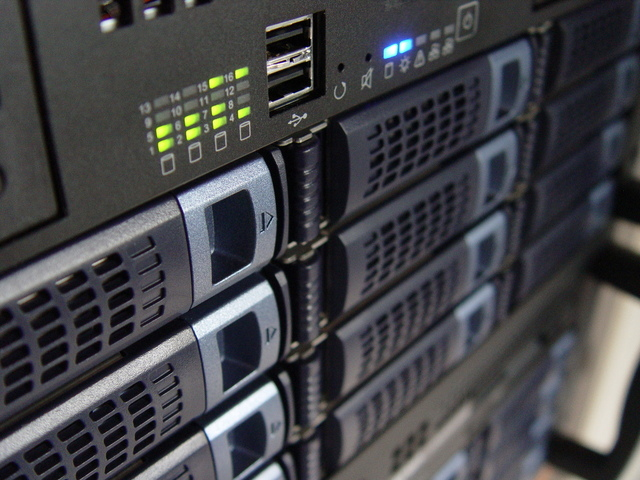
\includegraphics[scale=0.5]{servers.jpg}
}
\par\vspace{2cm}{
	Ultima fecha modificado: \today
}
\end{center}

% Indice
\clearpage
\section{Desarrollo}
Para esta practica haremos uso de la aplicación web que se utilizo previamente en la practica anterior de modo en que toda la parte de implementación y de ejecución del servidor REST esta en la anterior practica, mientras que para esta solo es necesario programar en Java para que esta aplicación consuma los metodos del servidor REST, destacando que en el archivo del servidor solo se le añadio unas lineas de código antes de concluir la clase para que tuviera una funcionalidad extra, así como al archivo HTML.
\section{Códigos}
\subsection{Funciones añadidas en Servicio.java}
\lstinputlisting[language=Java]{Servicio.java}
\subsection{Bloques añadidos en prueba.html}
\lstinputlisting[language=HTML]{prueba.html}
\subsection{Makefile}
\lstinputlisting[language=bash]{../Makefile}
\subsection{Cliente REST}
\lstinputlisting[language=Java]{../Teclado.java}
\lstinputlisting[language=Java]{../Usuario.java}
\lstinputlisting[language=Java]{../Cliente.java}
\section{Capturas}
\begin{center}
  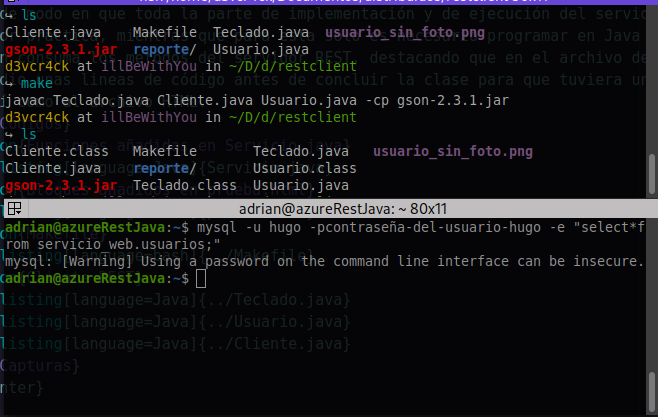
\includegraphics[scale=0.5]{imgs/com_sin_datos.png}
  \\\textit{Figura 1: Compilación de datos con el makefile y vistazo a que no tenga datos la app REST.}\\
  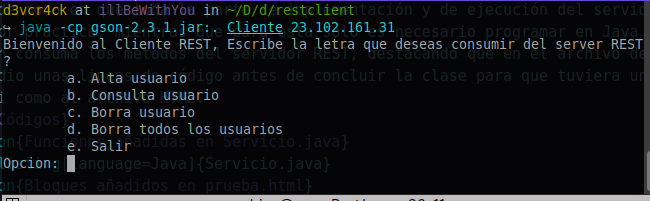
\includegraphics[scale=0.5]{imgs/menu.png}\\
  \textit{Figura 2: Menu solicitado para todas las tareas a realizar.}
  \\
  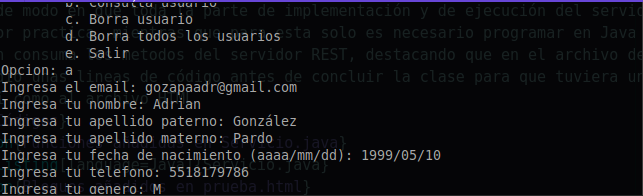
\includegraphics[scale=0.5]{imgs/alta.png}\\
  \textit{Figura 3: Alta de usuario.}
  \\
  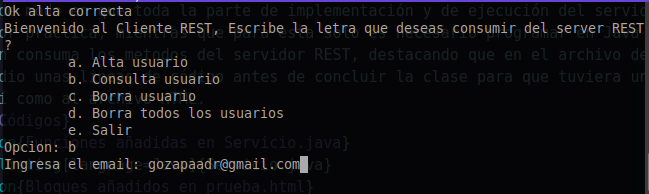
\includegraphics[scale=0.5]{imgs/alta-consulta.png}\\
  \textit{Figura 4: Mensaje de alta de usuario y consulta de existencia de esos datos.}
  \begin{landscape}
    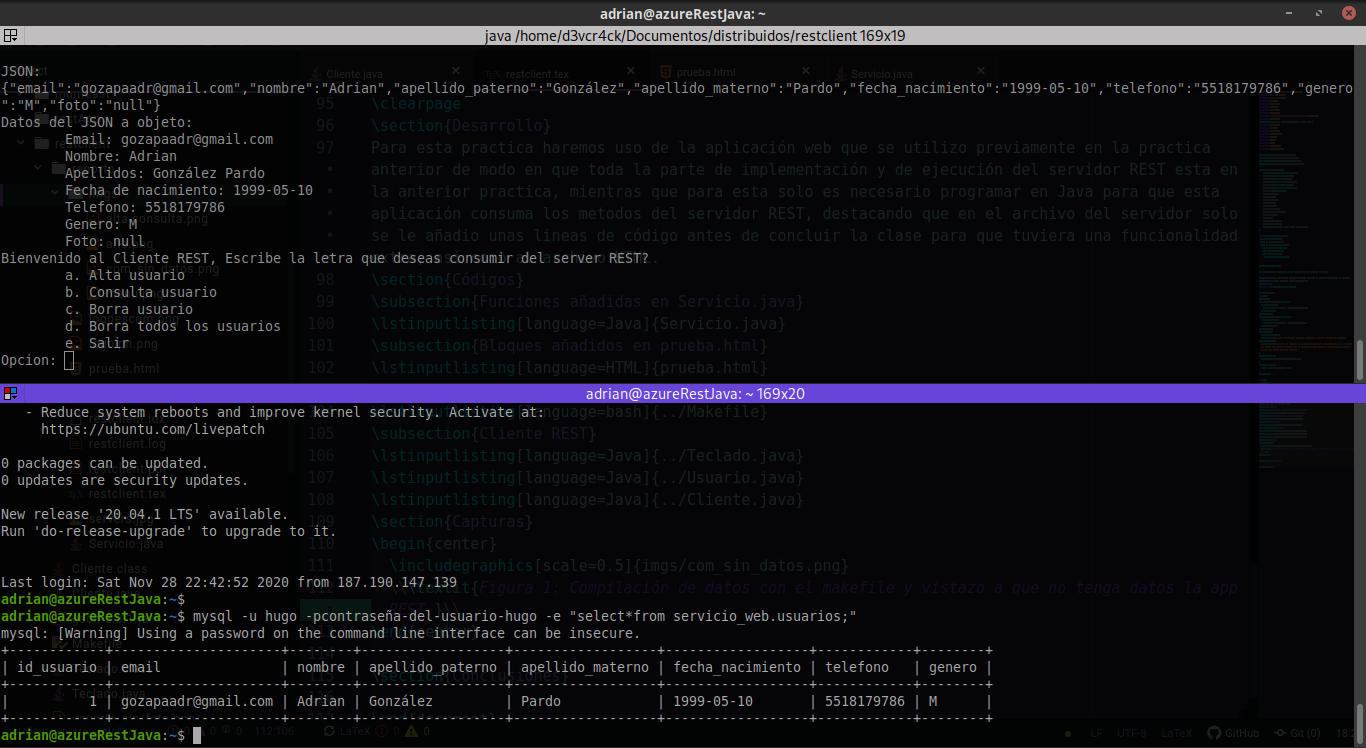
\includegraphics[scale=0.45]{imgs/consulta.png}\\
    \textit{Figura 5: Consulta tanto en BD y en aplicación.}
    \fillandplacepagenumber
  \end{landscape}
  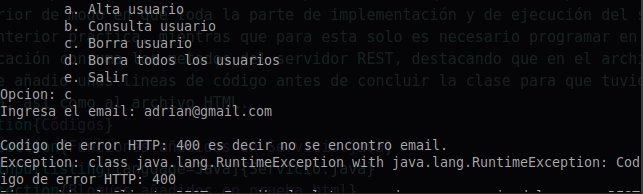
\includegraphics[scale=0.5]{imgs/del-not.png}\\
  \textit{Figura 6: Eliminación de un registro inexistente.}\\
  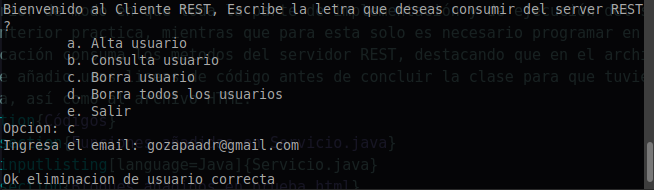
\includegraphics[scale=0.5]{imgs/del-correcta.png}\\
  \textit{Figura 7: Eliminación de un registro existente.}\\
  \begin{landscape}
    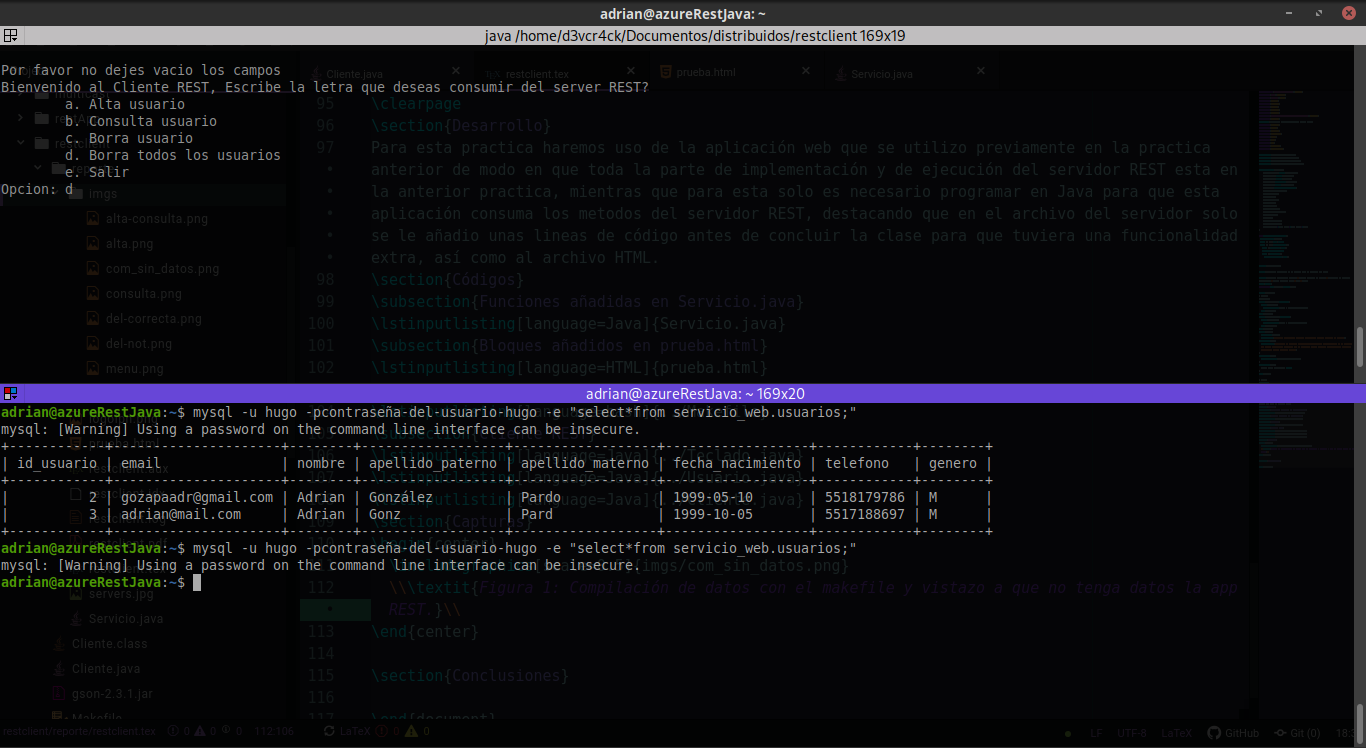
\includegraphics[scale=0.45]{imgs/del_all.png}\\
    \textit{Figura 8: Selección de eliminación de todos los registros de usuarios, más consulta en BD antes y despues de la petición.}
    \fillandplacepagenumber
  \end{landscape}
  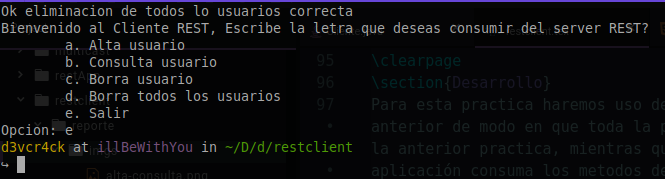
\includegraphics[scale=0.5]{imgs/msg_all.png}\\
  \textit{Figura 9: Mensaje de eliminación y opción de salida de la aplicación.}
\end{center}

\section{Conclusiones}
Programar esta aplicación fue realmente sencilla de modo en que la portabilidad de la misma es sencilla para trabajar ya que solo es pasar por parametro la IP del servidor para que el cliente pueda consumir, por otro lado este tipo de aplicaciones tambien puede ser trabajada com aplicaciones como cURL o incluso en otros lenguajes de programación ya que solo es realizar peticiones HTTP para REST.
\end{document}
